\subsection*{Extension}
One of the most important discussions of the paper I feel end ups falling short: what is the IV exercise actually identifying? The linear IV identification has several underlying assumption about the unobservable characteristics of the tribes. In this extension I will follow the theory described in \citet{Heckman05} and test some of the underlying assumptions that the author is imposing unobservables and discuss the implications on the authors estimations. 

Begin by considering the standard setting of potential outcomes \vspace{-18pt}
\begin{align*}
    Y_1 &= \mu_1(X) + U_1 \\ 
    Y_0 &= \mu_0(X) + U_0 \vspace{-13pt}
\end{align*}
and define $\Delta(X) = \mu_1(X)-\mu_0(X) + U_1-U_0$ the treatment effect conditional on observables. For the paper, we expect $\Delta(X)<0$. From the switch regression we can write \vspace{-18pt}
\begin{equation*}
    Y = \mu_0(X) + D\Delta(X) + U \vspace{-13pt}
\end{equation*}
To simplify the notation and make it consistent with \citet{Heckman05} denote by $J(Z,X)=\text{BLP}(D\vert X,Z)$ the first stage result conditional on $X$. Assuming that conditional on observables, the treatment effect is constant. implies that $U_1-U_0=0$ and thus $U_1=U_0=U$. Then the IV estimate conditional on $X$ is \vspace{-10pt}
\begin{align*}
    \frac{\text{Cov}(J(Z,X),Y\vert X)}{\text{Cov}(J(Z,X),D\vert X)} &= \frac{\text{Cov}(J(Z,X),\mu_0(X) + D\Delta(X) + U\vert X)}{\text{Cov}(J(Z,X),D\vert X)} \\ 
    &= \frac{\text{Cov}(J(Z,X),D\Delta(X) \vert X)}{\text{Cov}(J(Z,X),D\vert X)} \\
    &= \Delta(X) \vspace{-13pt}
\end{align*}
where the second line uses the instrument exogeneity and line three uses the assumption $U_1=U_0$ and thus $\Delta(X)$ is fully determined by $X$. However, dropping this assumption breaks the logic that IV is estimating the treatment effect. If we drop the assumption then IV is identifying \vspace{-13pt}
\begin{equation*}
    \frac{\text{Cov}(J(Z,X),Y\vert X)}{\text{Cov}(J(Z,X),D\vert X)} = \mu_1(X)-\mu_0(X) + \frac{\text{Cov}(J(Z,X),D(U_1-U_0) \vert X)}{\text{Cov}(J(Z,X),D\vert X)}
\end{equation*}
Instrument exogeneity implies that $J(Z,X)$ is independent from $U_1-U_0$ conditional on $X$. However it does not imply that $J(Z,X)$ is independent from $D(U_1-U_0)$. Thus, for IV to properly work, we need to impose one extra assumption, is that there is no sorting based on unobservables.

Given this, I want to test the assumption that there is no sorting based on unobservables. To do so, I will a result showed by \citet{Heckman05}: If there is no sorting, the the marginal treatment effect defined as 
\begin{equation*}
    \Delta^{\text{MTE}}(x,p) = \mathbb{E}\left[\Delta(X)\vert X=x, U_1-U_0=p\right]
\end{equation*}
is constant on $p$. Intuitively, if there is no sorting based on unobservables, then  changing  the set of unobservables should not change the treatment effect. Let $P(Z)$ be the propensity score of being treated. Using the results showed by \citet{Heckman05}
\begin{equation}\label{eq:func}
    \mathbb{E}[Y\vert P(Z)=p] = \mathbb{E}[Y_0] + \Delta^{\text{ATE}}p + \int_0^p\mathbb{E}[U_1-U_0\vert u_D]\mathrm{d}u_D
\end{equation}
By differentiating and using the Fundamental theorem of calculus
\begin{equation*}
    \frac{\partial\mathbb{E}[Y\vert P(Z)=p]}{\partial p} = \Delta^{\text{ATE}}+\mathbb{E}[U_1-U_0\vert p] = \Delta^{\text{MTE}}(p) 
\end{equation*}
Thus, a sufficient condition to claim there is no sorting based on unobservables is that $\mathbb{E}[Y\vert P(Z)=p]$ is linear on $p$. Recall that for a proper estimation of the propensity score, it is required a common support. I calculate the propensity score using both a probit and the predicted value from the first stage. The results are presented in Figure \ref{fig:comSupp}.
\begin{figure}[htb]
    \caption{\sc Common Support}
    \label{fig:comSupp}
    \begin{center}
     \begin{subfigure}[b]{0.47\textwidth}
         \centering
         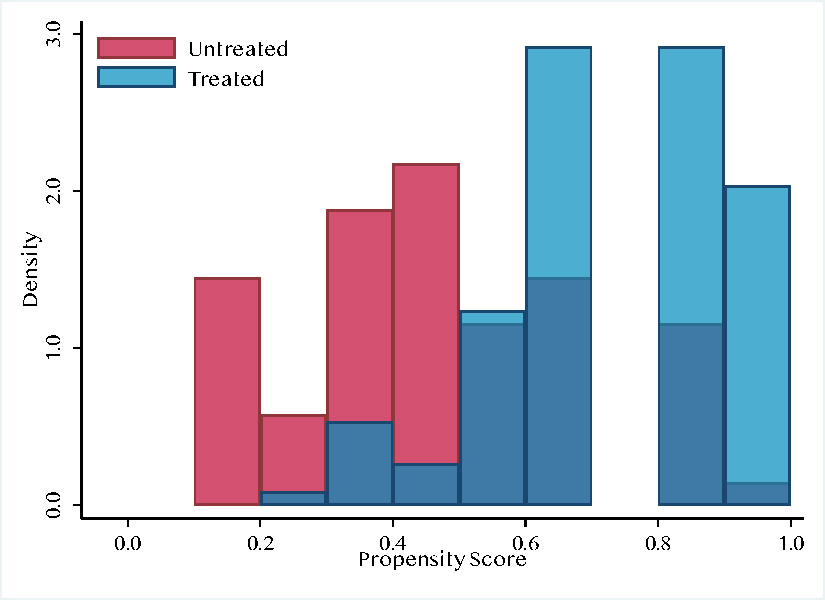
\includegraphics[width=\textwidth]{Figures/commonSupp.pdf}
         \caption{Probit}
     \end{subfigure}
     \begin{subfigure}[b]{0.47\textwidth}
         \centering
         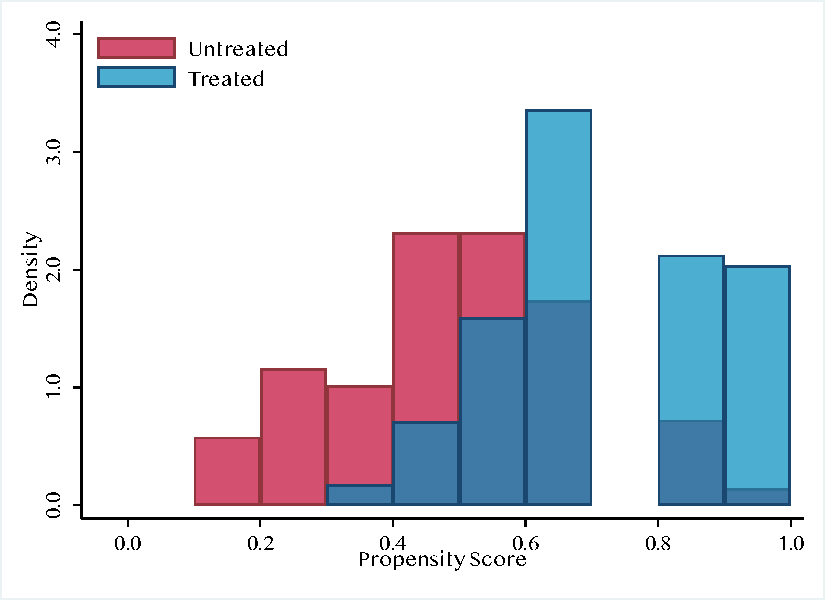
\includegraphics[width=\textwidth]{Figures/commonSuppLin.pdf}
         \caption{Linear Regression}
     \end{subfigure}
    \end{center}
    \vspace{-10pt}
    \scriptsize{}
\end{figure}
\FloatBarrier
Thus, for the analysis, the method of estimating the proensity score will matter. If done with the probit then the linearity should only consider data with $p\geq0.2$. If using the linear estimate, then the data that can be used for the analysis requires $p\geq 0.3.$. Next in Figure \ref{fig:linTest} we present the object described in equation \eqref{eq:func}. 
\begin{figure}[htb]
    \centering
    \caption{\sc Linear Test}
    \label{fig:linTest}
    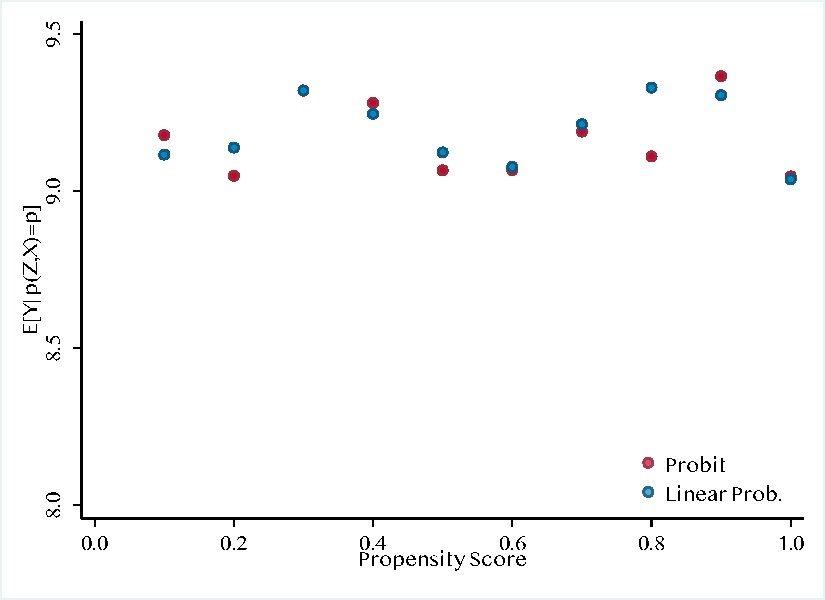
\includegraphics[width=0.48\textwidth]{Figures/Linear_Test.pdf}
\end{figure}
Upon inspection it is clear that there are some non-linearities and thus we can not discard the possibility of sorting based on unobservables. A more formal test could be performed following \citet{Chen1999}. 